\documentclass{article}
\usepackage[utf8]{inputenc}
\usepackage{hyperref}
\usepackage[letterpaper, portrait, margin=1in]{geometry}
\usepackage{enumitem}
\usepackage{amsmath}
\usepackage{booktabs}
\usepackage{graphicx}

\usepackage{titlesec}

\titleformat{\section}
{\normalfont\Large\bfseries}{\thesection}{1em}{}[{\titlerule[0.8pt]}]
  
\title{Homework 4 Answers}
\author{Economics 7103}
\date{ }
  
\begin{document}
  
\maketitle

\begin{enumerate}
\item See figure \ref{fig:hw4_q1}.  Yes, there appear to be parallel trends in fish bycatch for the treatment and control group before January 2018.  It appears that the program caused an immediate and large decline in bycatch.
\begin{figure}[h]
    \centering
    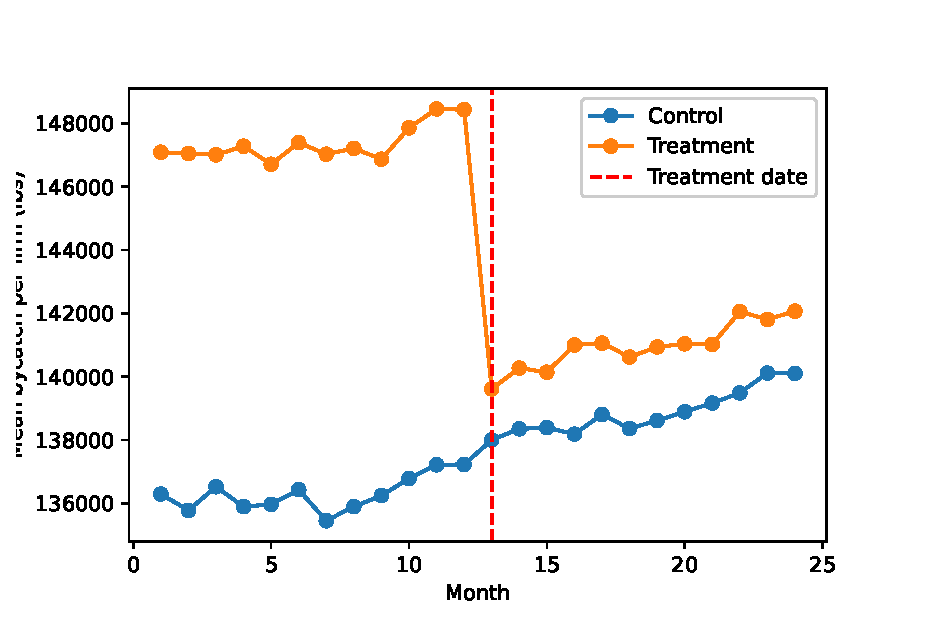
\includegraphics[scale = 0.7]{hw4_q1.eps}
    \caption{Plot showing mean firm bycatch in pounds for months in 2017 and 2018.  Treatment occurred in January 2018.}
    \label{fig:hw4_q1}
\end{figure}
\item The estimate is -9,591, which implies that between December and January the average bycatch per firm in the treated group declined by 9,591 pounds relative to firms in the control group over the same period.
\item Output displayed in table \ref{tab:hw4_output3}.  The result is equivalent to the result in 2 (as we would expect).
\end{enumerate}

\begin{table}[h]
    \centering
    \begin{tabular}{lc}
\toprule
{} &                    (3) \\
\midrule
Treatment group &                  11202 \\
                &  (-36028.81, 58432.89) \\
Treated         &               -9591.35 \\
                &  (-16085.87, -3096.83) \\
Pre-period      &                 773.22 \\
                &     (-429.89, 1976.32) \\
Constant        &                 137229 \\
                &  (99774.18, 174683.01) \\
Observations    &                    100 \\
\bottomrule
\end{tabular}

    \caption{Regression results for the two-period difference-in-differences estimation.  The estimate of interest is the coefficient on the ``Treated" variable. 95\% confidence intervals constructed using cluster-robust (at the firm level) standard errors.}
    \label{tab:hw4_output3}
\end{table}

\end{document}